\section{Vision Transformer (ViT): Biến Ảnh thành một Chuỗi các ''Từ''}
\label{sec:vision_transformer}

\subsection{Giới thiệu Tổng quan}
\label{subsec:vit_overview}
Năm 2020, một bài báo từ Google Research với tựa đề "An Image is Worth 16x16 Words" \cite{Dosovitskiy2020} đã tạo ra một cơn địa chấn trong cộng đồng thị giác máy tính. Bài báo này giới thiệu \textbf{Vision Transformer (ViT)}, mô hình đầu tiên chứng minh rằng một kiến trúc Transformer thuần túy, không có bất kỳ phép tích chập nào, có thể đạt được và thậm chí vượt qua hiệu năng của các mạng CNN state-of-the-art trong bài toán phân loại ảnh.

Chìa khóa cho thành công của ViT nằm ở hai yếu tố: một cách tiếp cận mới trong việc biểu diễn hình ảnh và quy mô dữ liệu huấn luyện khổng lồ. Thay vì nhìn một bức ảnh như một lưới pixel 2D cần được xử lý bằng các bộ lọc tích chập cục bộ, ViT đã áp dụng một triết lý triệt để từ NLP: nó coi một bức ảnh như một \textbf{chuỗi các "từ" thị giác}. Mỗi "từ" ở đây là một mảnh vá (patch) nhỏ của bức ảnh.

Bằng cách biến đổi bài toán từ xử lý không gian 2D sang xử lý chuỗi 1D, ViT đã mở đường cho cơ chế \textbf{self-attention} toàn cục của Transformer có thể được áp dụng trực tiếp. Điều này cho phép mô hình học được các mối quan hệ ngữ nghĩa phức tạp giữa các vùng ảnh xa nhau, một năng lực mà các mạng CNN phải rất vất vả mới đạt được một cách gián tiếp. Mặc dù ViT đòi hỏi một lượng dữ liệu huấn luyện cực lớn để có thể học các thiên kiến thị giác từ đầu, thành công của nó đã đánh dấu một bước ngoặt, mở ra một hướng đi hoàn toàn mới cho các kiến trúc thị giác.

\subsection{Kiến trúc Cốt lõi: Từ Lưới Pixel đến Chuỗi Token}
\label{subsec:vit_core_architecture}
Để một Transformer có thể "hiểu" được một bức ảnh, bước đầu tiên và quan trọng nhất là phải chuyển đổi nó từ dạng lưới pixel 2D sang dạng chuỗi các vector 1D (tokens) mà Transformer có thể xử lý.

\subsubsection{Bước 1: Patchification - Chia ảnh thành các Mảnh vá}
\label{subsubsec:vit_patchification}
Ảnh đầu vào, giả sử có kích thước $H \times W \times C$ (chiều cao $\times$ chiều rộng $\times$ số kênh), được chia thành một lưới các mảnh vá (patches) hình vuông, không chồng chéo. Mỗi patch có kích thước cố định là $P \times P$.
\begin{itemize}
	\item Số lượng patch thu được, $N$, được tính bằng:
	\begin{equation}
		N = \frac{H \times W}{P^2}
	\end{equation}
	\item Ví dụ, với một ảnh đầu vào tiêu chuẩn từ ImageNet có kích thước $224 \times 224$ và kích thước patch là $16 \times 16$, chúng ta sẽ có:
	\begin{equation}
		N = \frac{224 \times 224}{16 \times 16} = 14 \times 14 = 196 \text{ patches}
	\end{equation}
\end{itemize}
Kết quả của bước này là một chuỗi gồm 196 mảnh vá, mỗi mảnh có kích thước $16 \times 16 \times 3$.

\begin{center}
	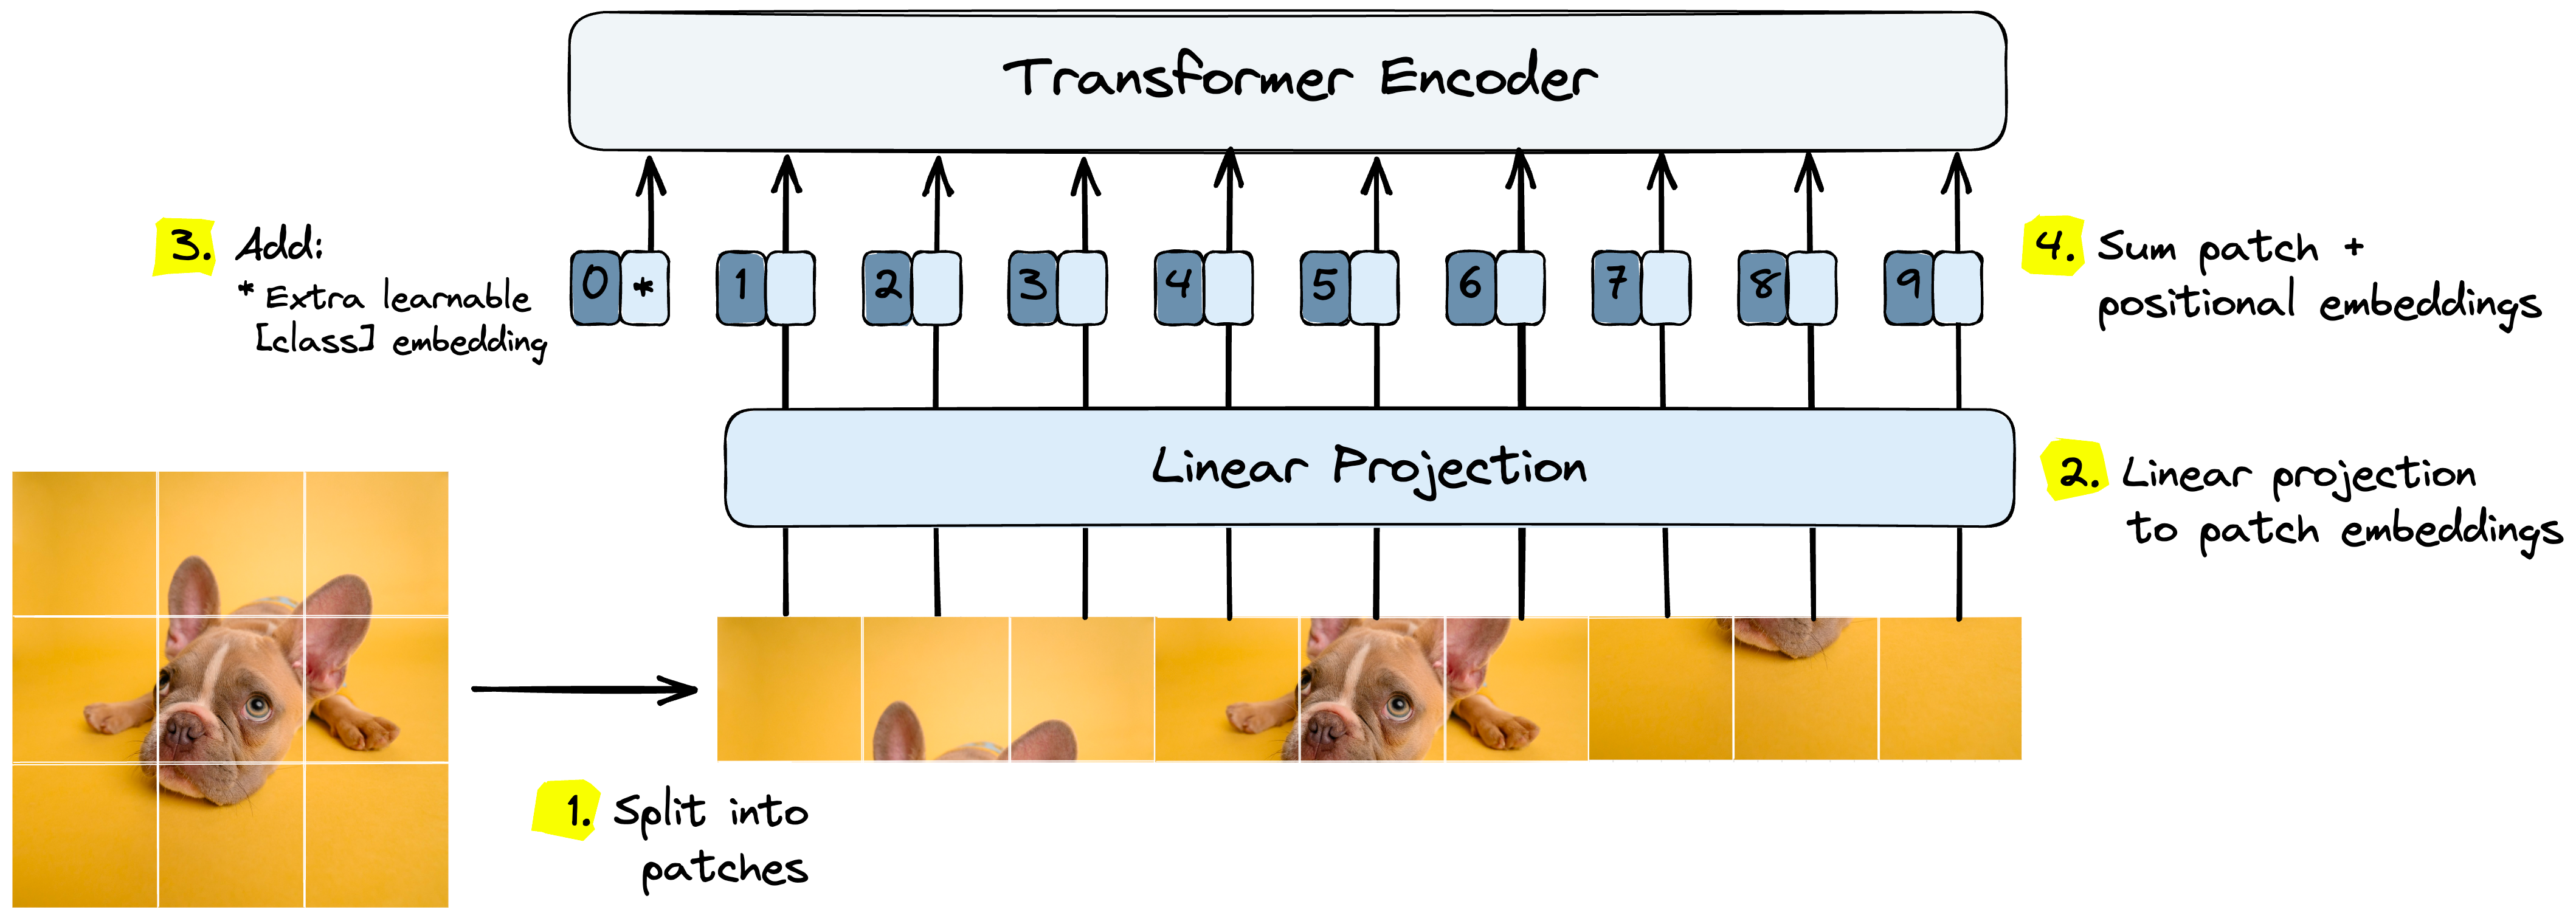
\includegraphics[width=0.8\textwidth]{images/vit_patching_process.png}
	\captionof{figure}{Quá trình "Patchification". Một ảnh đầu vào được chia thành một lưới các patch có kích thước cố định. Mỗi patch sẽ được coi như một "từ" trong chuỗi đầu vào của Transformer.}
	\label{fig:vit_patching}
\end{center}
% Keyword gợi ý: vision transformer patching, vit patch embedding diagram

\subsubsection{Bước 2: Patch Embedding - Dát phẳng và Chiếu tuyến tính}
\label{subsubsec:vit_patch_embedding}
Mỗi patch 2D sau đó được "dát phẳng" (flattened) thành một vector 1D.
\begin{itemize}
	\item Kích thước của vector này là $P \times P \times C$. Với ví dụ trên, kích thước là $16 \times 16 \times 3 = 768$.
	\item Sau đó, chuỗi các vector patch này được đưa qua một lớp \textbf{chiếu tuyến tính (linear projection)} có thể học được (về bản chất là một lớp fully-connected). Lớp này ánh xạ mỗi vector patch vào một không gian có chiều không đổi $D$, được gọi là \textbf{embedding dimension} (ví dụ, $D=768$ cho ViT-Base).
	\begin{equation}
		\mathbf{z}_p = \mathbf{x}_p \mathbf{E}
	\end{equation}
	trong đó $\mathbf{x}_p \in \mathbb{R}^{P^2 \cdot C}$ là vector patch đã được dát phẳng, và $\mathbf{E} \in \mathbb{R}^{(P^2 \cdot C) \times D}$ là ma trận embedding có thể học được.
\end{itemize}
Kết quả là một chuỗi gồm $N$ vector embedding, mỗi vector có chiều $D$. Đây chính là chuỗi các "token embedding" tương tự như trong NLP.

\subsubsection{Bước 3: Bổ sung [CLS] Token cho Phân loại}
\label{subsubsec:vit_cls_token}
Lấy cảm hứng từ kiến trúc BERT trong NLP, một token đặc biệt có thể học được, gọi là \textbf{[CLS] token} (viết tắt của Classification), được chèn vào đầu chuỗi các patch embedding.
\begin{itemize}
	\item Token này không tương ứng với bất kỳ patch nào của ảnh.
	\item Nó đi qua toàn bộ các lớp Transformer Encoder cùng với các patch embedding khác và tương tác với chúng thông qua cơ chế self-attention.
	\item \textbf{Mục đích:} Trạng thái cuối cùng của [CLS] token (vector embedding của nó ở output của Transformer Encoder) được coi là biểu diễn tóm tắt cho toàn bộ hình ảnh. Vector này sau đó sẽ được đưa qua một "đầu" phân loại (MLP Head) để đưa ra dự đoán cuối cùng.
\end{itemize}

\subsubsection{Bước 4: Mã hóa Vị trí (Positional Encoding)}
\label{subsubsec:vit_positional_encoding}
Một hạn chế cố hữu của cơ chế self-attention là nó có \textbf{tính hoán vị bất biến (permutation-invariant)}. Nó xử lý một tập hợp các token chứ không phải một chuỗi; nếu ta tráo đổi vị trí của các patch, output của self-attention sẽ thay đổi tương ứng nhưng mối quan hệ giữa chúng không đổi. Điều này có nghĩa là Transformer không có thông tin nội tại về vị trí của các patch.

Để khắc phục, thông tin về vị trí không gian phải được "tiêm" vào. ViT thực hiện điều này bằng cách cộng một \textbf{positional embedding} có thể học được vào mỗi patch embedding:
\begin{equation}
	\mathbf{z}_0 = [\mathbf{x}_{\text{class}}; \mathbf{x}_p^1 \mathbf{E}; \mathbf{x}_p^2 \mathbf{E}; \dots ; \mathbf{x}_p^N \mathbf{E}] + \mathbf{E}_{\text{pos}}
\end{equation}
trong đó:
\begin{itemize}
	\item $\mathbf{z}_0$ là chuỗi các embedding sẵn sàng đưa vào Transformer Encoder.
	\item $\mathbf{x}_{\text{class}}$ là embedding của [CLS] token.
	\item $\mathbf{E}_{\text{pos}} \in \mathbb{R}^{(N+1) \times D}$ là một ma trận embedding vị trí có thể học được. Mỗi hàng của nó tương ứng với một vị trí trong chuỗi (vị trí 0 cho [CLS] token, vị trí 1 cho patch đầu tiên, v.v.).
\end{itemize}
Trong quá trình huấn luyện, mạng sẽ tự học các embedding vị trí này để mã hóa thông tin về cấu trúc không gian của ảnh.

\subsubsection{Bước 5: Chuỗi Embedding Đầu vào Transformer Encoder}
\label{subsubsec:vit_input_to_encoder}
Sau khi đã thêm embedding vị trí, ta thu được một chuỗi gồm $(N + 1)$ vector embedding, mỗi vector có chiều $D$:
\begin{equation}
	\mathbf{Z}_0 = [\mathbf{z}_{\text{CLS}}, \mathbf{z}_1, \mathbf{z}_2, \dots, \mathbf{z}_N] \in \mathbb{R}^{(N+1) \times D}
\end{equation}
Chuỗi này được đưa vào khối \textbf{Transformer Encoder} nhiều tầng (thường gồm 12 tầng cho ViT-Base).  
Mỗi tầng bao gồm hai thành phần chính:
\begin{itemize}
	\item \textbf{Multi-Head Self-Attention (MHSA):} giúp mỗi patch “nhìn thấy” và tương tác với tất cả các patch khác trong ảnh.
	\item \textbf{Feed-Forward Network (FFN):} giúp trích xuất và biến đổi đặc trưng phi tuyến sau mỗi bước attention.
\end{itemize}
Tương tự như trong NLP, sau mỗi tầng encoder là các phép \textit{LayerNorm} và \textit{Residual Connection} giúp ổn định gradient.  
Kết quả cuối cùng, embedding của token [CLS] ở tầng cuối cùng $\mathbf{z}_{\text{CLS}}^{(L)}$ được dùng làm đặc trưng toàn cục của ảnh.

\subsection{Kiến trúc Tổng thể của ViT}
\label{subsec:vit_full_architecture}
Kiến trúc hoàn chỉnh của Vision Transformer (ViT) có thể được xem như một “phiên bản thị giác” của Transformer trong NLP, được điều chỉnh để xử lý dữ liệu hình ảnh. Nó bao gồm ba phần chính:

\begin{enumerate}
	\item \textbf{Embedding Layer:}  
	Thực hiện toàn bộ các bước từ \S\ref{subsubsec:vit_patchification} đến \S\ref{subsubsec:vit_positional_encoding}, tức là:
	\begin{itemize}
		\item Chia ảnh đầu vào thành các \textit{patch} kích thước cố định ($P \times P$).
		\item Dát phẳng và chiếu mỗi patch vào không gian có chiều $D$ để tạo ra các \textit{token embedding}.
		\item Bổ sung token đặc biệt [CLS] và thông tin vị trí thông qua \textit{positional embedding}.
	\end{itemize}
	Kết quả là một chuỗi $(N + 1)$ token embedding, sẵn sàng được đưa vào phần Transformer Encoder.
	
	\item \textbf{Transformer Encoder:}  
	Đây là phần lõi của mô hình và cũng là nơi thực hiện việc trích xuất đặc trưng toàn cục. Nó bao gồm $L$ lớp (block) Transformer Encoder xếp chồng lên nhau (thường $L=12$ cho ViT-Base, $L=24$ cho ViT-Large).  
	Mỗi lớp gồm hai khối con chính:
	\begin{itemize}
		\item \textbf{Multi-Head Self-Attention (MHSA):} Cho phép mỗi patch “nhìn thấy” tất cả các patch khác trong ảnh, nhờ đó mô hình có thể học được các mối quan hệ toàn cục — điều mà CNN truyền thống (với kernel cục bộ) phải cần rất nhiều tầng để đạt được.
		\item \textbf{Feed-Forward Network (FFN):} Một MLP áp dụng độc lập trên từng token, giúp mô hình học các biến đổi phi tuyến sau khi trộn thông tin qua self-attention.  
		FFN thường gồm hai lớp tuyến tính:
		\begin{equation}
			\text{FFN}(x) = W_2 \cdot \text{GELU}(W_1 x + b_1) + b_2
		\end{equation}
	\end{itemize}
	Cả hai khối con này đều được bao quanh bởi các \textbf{kết nối tắt (residual connection)} và \textbf{chuẩn hóa lớp (Layer Normalization)}, giúp ổn định gradient và cải thiện khả năng hội tụ trong huấn luyện.
	
	\item \textbf{MLP Head:}  
	Một \textit{head} phân loại nhỏ (thường gồm một hoặc hai lớp tuyến tính) được đặt ở cuối. Nó nhận đầu vào là embedding của [CLS] token sau khi đi qua tất cả các tầng encoder:
	\begin{equation}
		\hat{y} = \text{softmax}(W_{\text{cls}} \cdot \mathbf{z}_{\text{CLS}}^{(L)} + b_{\text{cls}})
	\end{equation}
	Vector $\mathbf{z}_{\text{CLS}}^{(L)}$ được xem là biểu diễn trừu tượng toàn cục của ảnh, tương tự như “feature vector” ở đầu cuối của một CNN.
\end{enumerate}

\begin{center}
	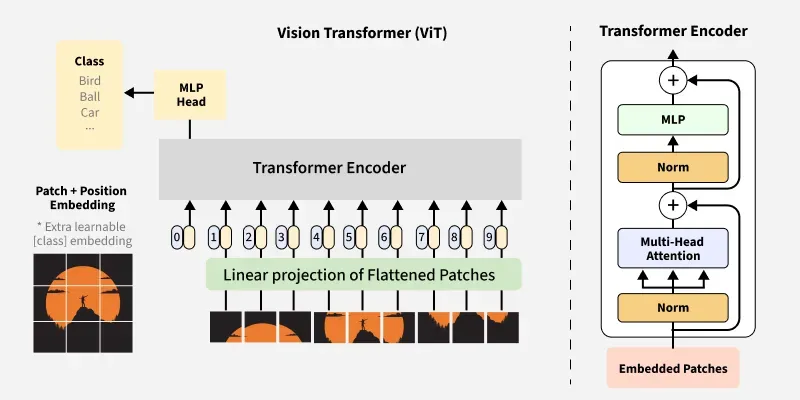
\includegraphics[width=1.0\textwidth]{images/vision_transformer_vit_architecture.png}
	\captionof{figure}{Sơ đồ kiến trúc tổng thể của Vision Transformer (ViT). Ảnh được chia thành các patch, được nhúng và bổ sung thông tin vị trí. Chuỗi các vector này sau đó được xử lý bởi nhiều tầng Transformer Encoder. Cuối cùng, vector [CLS] được dùng để phân loại.}
	\label{fig:vit_architecture}
\end{center}

\subsubsection*{Bình luận: Ưu điểm và Hạn chế của Kiến trúc ViT}
ViT đã chứng minh rằng Transformer có thể cạnh tranh (thậm chí vượt qua) CNN trên các bộ dữ liệu lớn như ImageNet. Tuy nhiên, kiến trúc này cũng có những đặc điểm riêng đáng chú ý:
\begin{itemize}
	\item \textbf{Ưu điểm:}
	\begin{itemize}
		\item Mối quan hệ toàn cục được mô hình hóa trực tiếp thông qua self-attention, giúp nắm bắt các phụ thuộc dài hạn trong không gian hình ảnh.
		\item Kiến trúc đơn giản và thống nhất: chỉ cần stack các block Transformer, không cần thiết kế thủ công các khối tích chập phức tạp.
		\item Dễ mở rộng quy mô (scalable) khi tăng số tầng hoặc số chiều embedding.
	\end{itemize}
	\item \textbf{Hạn chế:}
	\begin{itemize}
		\item Thiếu \textit{inductive bias} cục bộ vốn có trong CNN, nên cần lượng dữ liệu lớn và huấn luyện mạnh để đạt hiệu năng cao.
		\item Tốn bộ nhớ và thời gian tính toán do cơ chế attention có độ phức tạp $O(N^2)$ theo số lượng patch.
	\end{itemize}
\end{itemize}
Những hạn chế này đã mở đường cho các biến thể tiếp theo như \textbf{DeiT}, \textbf{Swin Transformer}, và \textbf{ConvNeXt}, nơi các nghiên cứu tìm cách kết hợp ưu điểm của cả CNN và Transformer.

\subsection{Phân tích Ưu điểm và Hạn chế}
\label{subsec:vit_pros_cons}
Sau khi hiểu rõ cấu trúc và nguyên lý hoạt động của ViT, phần này trình bày những ưu điểm nổi bật và hạn chế còn tồn tại của kiến trúc này.

\subsubsection{Ưu điểm}
\label{subsubsec:vit_advantages}
\begin{itemize}
	\item \textbf{Khả năng Mô hình hóa Quan hệ Toàn cục:} Đây là ưu điểm then chốt. Nhờ cơ chế self-attention, ViT có thể nắm bắt các phụ thuộc tầm xa giữa các vùng khác nhau trong ảnh, giúp mô hình hiểu được bối cảnh và cấu trúc tổng thể tốt hơn so với CNN vốn chủ yếu dựa trên quan hệ cục bộ.
	\item \textbf{Khả năng Mở rộng (Scalability):} Hiệu năng của ViT tăng gần như tuyến tính khi tăng kích thước mô hình (ViT-Base, ViT-Large, ViT-Huge) và quy mô dữ liệu huấn luyện. Điều này khiến ViT đặc biệt phù hợp trong kỷ nguyên các mô hình nền tảng (foundation models) quy mô cực lớn.
	\item \textbf{Thiên kiến Quy nạp ít hơn (Less Inductive Bias):} ViT không bị ràng buộc bởi các giả định cứng nhắc về tính cục bộ hay bất biến tịnh tiến như trong CNN. Điều này giúp mô hình linh hoạt hơn, có khả năng học được các quy luật phi truyền thống từ dữ liệu, dù phải đánh đổi bằng yêu cầu dữ liệu lớn hơn.
\end{itemize}

\subsubsection{Hạn chế}
\label{subsubsec:vit_disadvantages}
\begin{itemize}
	\item \textbf{"Đói" Dữ liệu (Data-Hungry):} Do thiếu các thiên kiến quy nạp tự nhiên về tính cục bộ và bất biến tịnh tiến như trong CNN, ViT cần một lượng dữ liệu khổng lồ để học các quy luật thị giác cơ bản từ đầu. Khi huấn luyện trên các bộ dữ liệu quy mô trung bình như ImageNet-1K (1.2 triệu ảnh), ViT thuần túy thường cho hiệu năng kém hơn các mạng ResNet tương đương. Sức mạnh của nó chỉ thực sự bộc lộ khi được huấn luyện trước trên các bộ dữ liệu rất lớn như JFT-300M (300 triệu ảnh) của Google.
	\item \textbf{Độ phức tạp Tính toán:} Cơ chế self-attention có độ phức tạp $O(N^2)$ theo số lượng patch. Điều này khiến chi phí tính toán và bộ nhớ tăng nhanh khi độ phân giải ảnh cao, làm hạn chế việc áp dụng trực tiếp ViT cho các tác vụ yêu cầu độ phân giải lớn.
\end{itemize}


\subsection{Tác động và Di sản}
\label{subsec:vit_impact_legacy}
Sự ra đời của ViT đánh dấu một bước ngoặt trong thị giác máy tính, khi lần đầu tiên một mô hình Transformer thuần túy có thể cạnh tranh (và thậm chí vượt qua) các mạng CNN truyền thống trên quy mô lớn. ViT đã khởi đầu một làn sóng nghiên cứu mạnh mẽ với nhiều hướng cải tiến và mở rộng:

\begin{itemize}
	\item \textbf{DeiT (Data-efficient Image Transformer)} \cite{Touvron2021}: Đề xuất các kỹ thuật huấn luyện hiệu quả hơn, như chưng cất tri thức (knowledge distillation), giúp ViT đạt hiệu năng cao ngay cả khi chỉ huấn luyện trên ImageNet-1K.
	\item \textbf{Swin Transformer} \cite{Liu2021}: Tái giới thiệu thiên kiến cục bộ bằng cách tính toán self-attention trong các cửa sổ (windows) chồng lấn, giúp giảm chi phí $O(N^2)$ xuống gần mức tuyến tính và tăng khả năng mở rộng cho các tác vụ có độ phân giải cao.
\end{itemize}

Quan trọng hơn, ViT đã chứng minh rằng kiến trúc Transformer là một "ngôn ngữ chung" có thể áp dụng cho nhiều dạng dữ liệu khác nhau. Di sản của nó mở đường cho các mô hình đa phương thức và nền tảng (foundation models), cũng như các ứng dụng mở rộng trong phát hiện vật thể (DETR), phân đoạn ảnh (Segmenter), và thậm chí trong mô hình thị giác–ngôn ngữ (Vision–Language Models).

\section*{Tài liệu tham khảo}
\begin{itemize}
	\item[1] Dosovitskiy, A., Beyer, L., Kolesnikov, A., Weissenborn, D., Zhai, X., Unterthiner, T., ... \& Houlsby, N. (2020). An image is worth 16x16 words: Transformers for image recognition at scale. \textit{arXiv preprint arXiv:2010.11929}. (Paper gốc giới thiệu Vision Transformer - ViT).
	\item[2] Vaswani, A., Shazeer, N., Parmar, N., Uszkoreit, J., Jones, L., Gomez, A. N., ...\& Polosukhin, I. (2017). Attention is all you need. In \textit{Advances in neural information processing systems (NIPS)}. (Paper gốc giới thiệu kiến trúc Transformer trong NLP, nền tảng của ViT).
	\item[3] Devlin, J., Chang, M. W., Lee, K.,\& Toutanova, K. (2018). Bert: Pre-training of deep bidirectional transformers for language understanding. \textit{arXiv preprint arXiv:1810.04805}. (Giới thiệu mô hình BERT và việc sử dụng [CLS] token cho các tác vụ phân loại).
	\item[4] Touvron, H., Cord, M., Douze, M., Massa, F., Sablayrolles, A.,\& Jégou, H. (2021). Training data-efficient image transformers\& distillation through attention. In \textit{International Conference on Machine Learning (ICML)}. (Giới thiệu DeiT).
	\item[5] Liu, Z., Lin, Y., Cao, Y., Hu, H., Wei, Y., Zhang, Z., ...\& Guo, B. (2021). Swin transformer: Hierarchical vision transformer using shifted windows. In \textit{Proceedings of the IEEE/CVF International Conference on Computer Vision (ICCV)}. (Giới thiệu Swin Transformer).
\end{itemize}